\documentclass[11pt]{article}
\usepackage[margin=1in, lmargin=0.75in]{geometry}
\usepackage{caption}
\usepackage{float}
\usepackage{graphicx}
\usepackage{latexsym}
\usepackage{amsmath}
\usepackage{cancel}
\usepackage{astro}
\usepackage{url}
\usepackage[bottom]{footmisc}

\newcommand\allbold[1]{{\boldmath\textbf{#1}}}
\newcommand\pc{\mathrm{\ pc}}
\newcommand\Lpc{\ L_\odot/\!\!\pc^2}
\newcommand\sech{\ \!\mathrm{sech}}
\newcommand\density{\left( \frac{M}{R^3} \right)}
\newcommand\kideal{K_\mathrm{ideal}}

\begin{document}

\begin{flushright}Meredith Durbin\\
Tom Quinn\\
Astro 507: Thermodynamics\\
\today\\

\end{flushright}

\center{\textsc{Homework 4}} \\[6pt]

\begin{enumerate}

\item
	\begin{enumerate}
    \item In the one-zone model, $P_c \sim GM^2/R^4$. We also assume $\rho \sim M/R^3$.
    \begin{align}
    \frac{GM^2}{R^4} &= \kideal\density T + K_e\density^{5/3} - K_C\density^{4/3} \\
    G &= \kideal M^{-1}RT + K_e M^{-1/3} R^{-1} - K_C M^{-2/3} \\ 
    R &= \frac{GM + K_CM^{1/3} - \sqrt{ (K_C M^{1/3} + GM)^2 - 4\kideal K_e M^{2/3} T } }{2\kideal T}
    \end{align}
    
    \item Plot of radius as a function of mass:
    \begin{figure}[H]
    \centering
    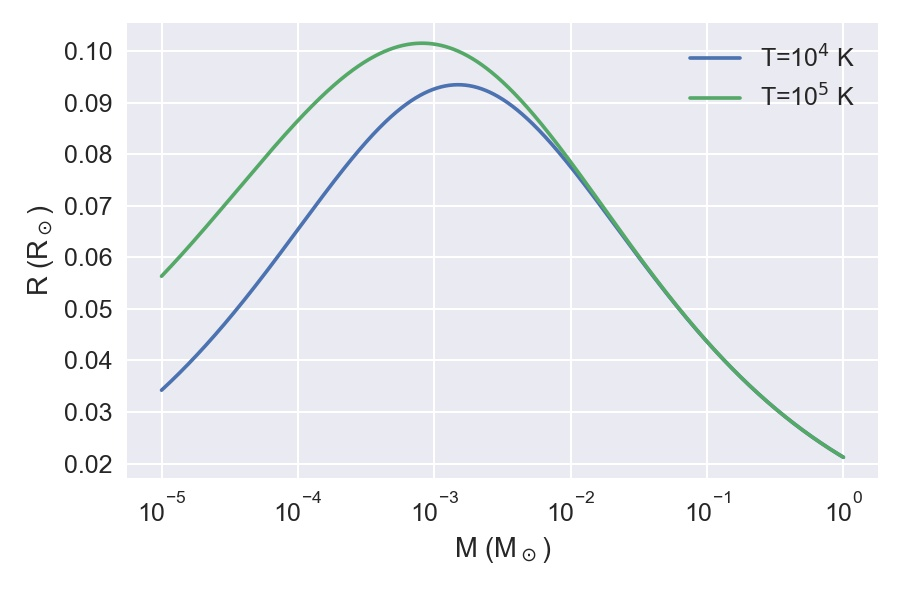
\includegraphics[width=0.7\textwidth]{mass_radius.jpg}
    \end{figure}
    
    \item I don't really understand what's meant by branches, but when the temperature is increased to $10^5$ K everything blows up below $\sim\!10^{-3.5}~M_\odot$. %I assume that ``branches" refers to the radii above and below the turning point near $10^{-3}~\mathrm{M}_\odot$.
    \end{enumerate}
    
\item The maximum mass of a degenerate neutrino ball is $M_\mathrm{max} \approx (\hbar c / G)^{3/2} m_\nu^{-2}$. Plot of $M_\mathrm{max}$ as a function of neutrino mass:
    \begin{figure}[H]
    \centering
    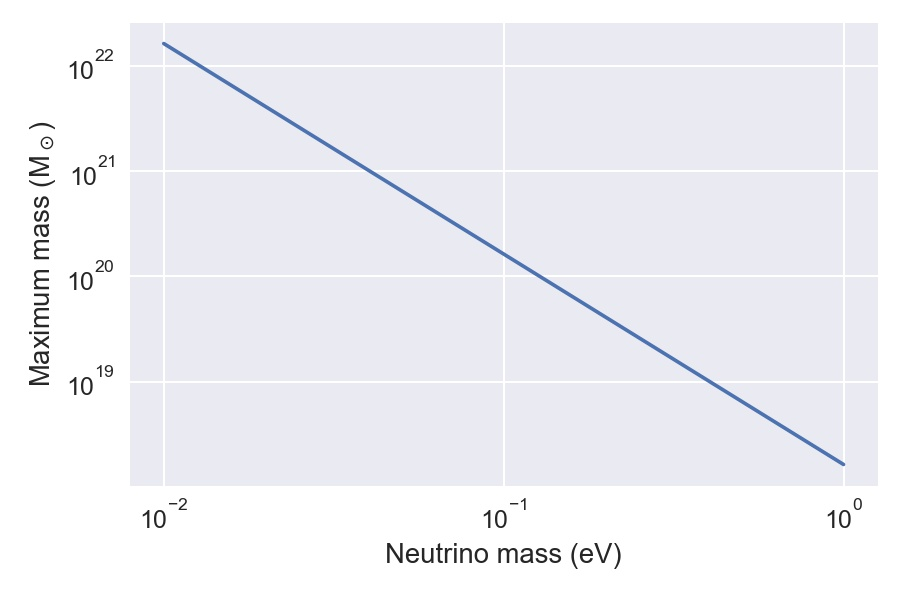
\includegraphics[width=0.7\textwidth]{neutrino.jpg}
    \end{figure}
    For a maximum black hole mass of $4 \times 10^9~M_\odot$, the requisite neutrino mass is 
20.2 keV, which is not at all consistent with the known neutrino mass upper limit. The mass is related to the radius by $R \approx h^2/(m_\nu^{8/3}G) M^{-1/3}$, which for $M_{BH} = 4 \times 10^9~M_\odot$ and $m_\nu = 0.1$ eV gives a radius of approximately $1\times10^{12}$ pc, which seems somewhat unreasonable. For a 20 keV neutrino, the black hole radius is 1559 AU, which is still on the unreasonable side.

\end{enumerate}
\end{document}